\renewcommand{\theequation}{\theenumi}
\begin{enumerate}[label=\arabic*.,ref=\thesubsubsection.\theenumi]
\numberwithin{equation}{enumi}
\item Solve the following system of linear inequalities graphically.
\begin{align}
\label{eq:line_two_ineq}
\begin{split}
    x &\geq 3
\\
    y &\geq 2
\end{split}
\end{align}
Let $u_1 \ge 0, u_2 \ge 0$.  This may be expressed as
\begin{align}
\vec{u} = \myvec{u_1\\u_2}\succeq \vec{0}
\end{align}
%
\eqref{eq:line_two_ineq} can then be expressed as
\begin{align}
\begin{split}
    x &\geq 5
\\
    y &\geq 2
\end{split}
%
\\
\implies 
\myvec{1 & 0 \\ 0 & 1}\vec{x}  &\succeq \myvec{5\\2}
\\
\myvec{1 & 0 \\ 0 & 1}\vec{x}  -\vec{u}&=\myvec{5\\2}
\\
\text{or, }
\myvec{1 & 0 \\ 0 & 1}\vec{x} &= \myvec{5\\2} +\vec{u}
\end{align}
%
resulting in 
\begin{align}
\vec{x} &= \myvec{1 & 0 \\ 0 & 1}^{-1}\myvec{5\\2} +\myvec{1 & 0 \\ 0 & 1}^{-1}\vec{u}
\\
\text{or, } \vec{x} &= \myvec{5\\2} +\myvec{1 & 0 \\ 1 & 0}\vec{u}
\end{align}
%
after obtaining the  inverse.
%
 Fig. \ref{fig:line_ineq} generated using the following python code shows the region satisfying \eqref{eq:line_two_ineq}

\begin{lstlisting}
codes/line/line_eq.py
\end{lstlisting}
%
\begin{figure}[!ht]
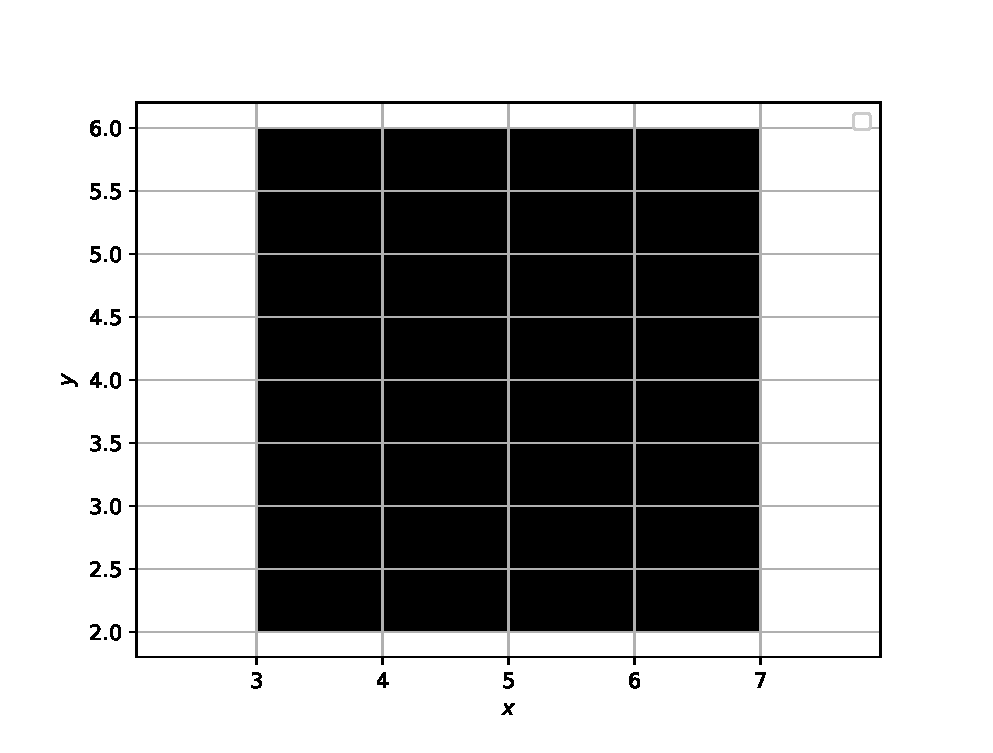
\includegraphics[width=\columnwidth]{./figs/line/line_eq.eps}
\caption{}
\label{fig:line_ineq}
\end{figure}
%



\end{enumerate}